\documentclass{article}
\usepackage[utf8]{inputenc}
\usepackage{amsmath}
\usepackage{amssymb}
\usepackage{amssymb}
\usepackage{upgreek}
\usepackage[colorlinks = true,
linkcolor = black,
urlcolor  = blue]{hyperref}

\usepackage[margin=1.5in]{geometry}
\usepackage{relsize}
\usepackage{color}
\usepackage{graphicx}
\usepackage{subcaption}
\usepackage{longtable}

\title{APMA 2822b Homework 4}
\author{Ryan Greenblatt}
\date{April 2019}

\begin{document}

\setlength\parindent{0pt}

\renewcommand{\thesubsection}{\alph{subsection}}

\maketitle

\section{}

Code is attached in the email. I have included a CMakeLists.txt file which can 
be used to compile the code on the CCV. The \verb cuda/9.1.85.1  module must be 
loaded. CUDA 10 also works, but results in errors when using nvprof.
I also added the SLURM scripts I used.

\subsection*{Algorithm and Implementation}

I implemented sparse matrix vector multiplication using the CRS and ELLPACK
data formats. The ELLPACK data format constructs a dense matrix with the same
number of rows as the sparse matrix and as many columns as the maximum number
of non-zero elements in the sparse matrix. As such, the data format performs well
when the number of non-zeros in most rows is close to the maximum number of
non-zeros. This provided sparse matrix is well suited to the ELLPACK data
format because the maximum number of non-zeros in a column (87) is very close to
the average number of non-zeros (54.8). The ELLPACK data format takes the
non-zero elements in each row and packs them into this dense
matrix. The column indexes of the entires are recorded in another dense matrix
with the same shape. To perform multiplication, each entry in the dense matrix
may be looped through and multiplied by the corresponding element in the vector.
The matrix of indexes is used to determine which vector element to use. 
I also stored the number of elements in each row and only looped through
that many elements as a further optimization. Additionally, the cuSPARSE
library was used for comparison.
Specifically, I tested using \texttt{cusparseDcsrmv} which operates on data in
the CRS format.  Both approaches were evaluated on the CPU, and on the 
GPU using both unified and device only memory.  I attempted to optimize the
ELLPACK implementation which doesn't use managed memory in two other ways.
I stored the vector in texture memory, which
improves mostly random, but spatially local data access. Hypothetically, this
is advantageous because each a group of threads will be operating on the same
part of the vector at once. I also used
\texttt{cudaMallocPitch} to allocate the 2D index and matrix arrays. This
pads 2D arrays to ensure proper alignment.  \\


\section{Results}

All testing was done on the CCV with a GPU (TITAN V) and a CPU core. 
Time required to copy data and convert between formats
wasn't counted. I ran each test 10 times and timed each run individually
so that the start up memory transfer cost for each approach could be evaluated.
Results are report in terms of the time required for one iteration of the
provided matrix.
The exact time and GLOPS of the computation will depend on the characteristics of the
sparse matrix. \\

As should be expected, the cuSPARSE implementation was the fastest. Surprising,
the standard CRS implementation was almost as fast and the ELLPACK
implementation was slower than both. Storing the number of elements in each
row and only looping through the required elements didn't improve performance.
Using a texture and \texttt{cudaMallocPitch} also resulted in no improvement.
The timing results can be seen in tables 1 and 2 below. Hypothetically,
the ELLPACK data format should have allowed for better vectorization and
more contiguous memory access. However, this doesn't appear to be the case.
Each thread iterated over a row, so perhaps the number of non-zeros in each
row was too small to yield a performance improvement. \\ 

Unified and device memory
had similar performance after the first iteration. The first
iteration using managed memory which switched from the CPU to GPU was
substantially slower because the managed memory needed to be
transfered from device to host. \\

Interestingly, the average kernel timings reported by nvprof were substantially
different from the timing found by the code. I used the CUDA event API to
time CUDA kernels in the code. I tested on both my laptop and the CCV and the disparity
wasn't at all present on my laptop. The average kernels durations as reported
by nvprof are given in table 3 below. I think that most likely the
kernel timings reported by nvprof are incorrect and the issue may be related
to the nvprof error which using CUDA 10. The issue may also be occurring in CUDA
9, but isn't properly reported.  \\ 

Profiling the code using nvprof allowed for detailed inspection of the time
required for each CUDA API call. The timings for each CUDA API call are given
in table 4 below. \texttt{cudaFree} was found to use
a large percentage of the overall time of the program (808.70 ms). It isn't
clear to me why this would be the case. \texttt{cudaMalloc}, 
\texttt{cudaMallocManaged}, and \texttt{cudaMallocPitch}
also took substantial program execution time. \texttt{cudaMemcpy} consumed
most of the remaining time spent on CUDA API calls. \\

\begin{figure}[h]
  \centering
  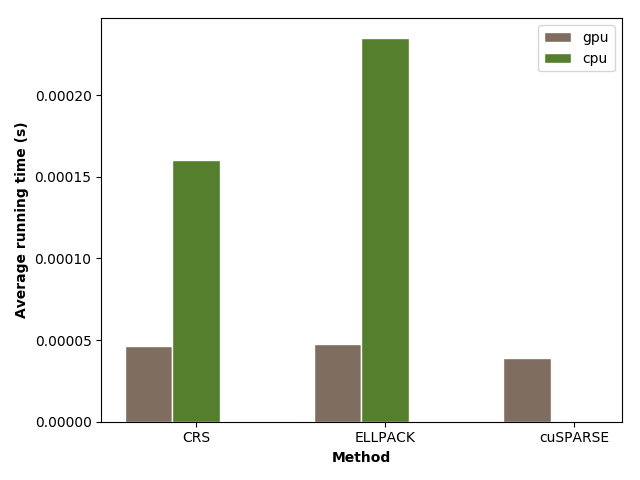
\includegraphics[width=0.8\linewidth]{running_times.png}
  \label{fig:running_times}
\end{figure}


\begin{table}[]
  \centering
  \begin{tabular}{|l|l|l|l|l|}
    \hline
    Method                 & Average time & 1            & 2            & 3            \\ \hline
    CPU                    & 1.163711e-03 & 1.230508e-03 & 1.182623e-03 & 1.163417e-03 \\ \hline
    GPU                    & 5.627600e-05 & 1.386880e-04 & 5.836800e-05 & 5.760000e-05 \\ \hline
    CPU managed before GPU & 1.147507e-03 & 1.383997e-03 & 1.390982e-03 & 1.314569e-03 \\ \hline
    GPU managed            & 5.724400e-05 & 3.816096e-03 & 6.208000e-05 & 5.772800e-05 \\ \hline
    CPU managed after GPU  & 1.147507e-03 & 1.383997e-03 & 1.390982e-03 & 1.314569e-03 \\ \hline
    cuSPARSE               & 4.769600e-05 & 1.735040e-04 & 5.174400e-05 & 4.816000e-05 \\ \hline
  \end{tabular}
  \caption{The recorded timings for each method utilizing the CRS data format.
    The average is the average over the 10 runs excluding the first two runs.
    Only the first 3 runs are shown to highlight transfer times associated with
  managed memory.}
\end{table}

\begin{table}[]
  \centering
  \begin{tabular}{|l|l|l|l|l|}
    \hline
    Method                 & Average time & 1            & 2            & 3            \\ \hline
    CPU                    & 1.532791e-03 & 1.666157e-03 & 1.545466e-03 & 1.527803e-03 \\ \hline
    GPU                    & 7.177600e-05 & 1.217280e-04 & 7.216000e-05 & 7.225600e-05 \\ \hline
    CPU managed before GPU & 1.717457e-03 & 1.943428e-03 & 1.957182e-03 & 1.930350e-03 \\ \hline
    GPU managed            & 7.079600e-05 & 6.245120e-03 & 7.136000e-05 & 6.908800e-05 \\ \hline
    CPU managed after GPU  & 1.717457e-03 & 1.943428e-03 & 1.957182e-03 & 1.930350e-03 \\ \hline
  \end{tabular}

  \caption{The recorded timings for each method utilizing the ELLPACK data
    format.
    The average is the average over the 10 runs excluding the first two runs.
    Only the first 3 runs are shown to highlight transfer times associated with
  managed memory.}
\end{table}

\begin{table}[]
  \centering
  \begin{tabular}{|l|l|}
    \hline
    Method                 & Average kernel time \\ \hline
    ELLPACK managed memory & 1.1221ms            \\ \hline
    CRS                    & 236.69us            \\ \hline
    ELLPACK                & 65.046us            \\ \hline
    cuSPARSE               & 38.012us            \\ \hline
  \end{tabular}
  \caption{The average running time of each kernel as reported by nvprof.
    I think these timings are likely wrong.}
\end{table}

\begin{table}[]
  \centering
  \begin{tabular}{|l|l|}
    \hline
    API Call                & Total time \\ \hline
    cudaFree                & 808.70ms   \\ \hline
    cudaMalloc              & 356.46ms   \\ \hline
    cudaMemcpy              & 26.645ms   \\ \hline
    cudaMallocManaged       & 20.576ms   \\ \hline
    cudaEventSynchronize    & 13.659ms   \\ \hline
    cudaDeviceSynchronize   & 5.7463ms   \\ \hline
    cudaMemcpy2D            & 4.6235ms   \\ \hline
    cuDeviceGetAttribute    & 995.13us   \\ \hline
    cudaLaunch              & 523.47us   \\ \hline
    cudaMallocPitch         & 359.52us   \\ \hline
    cudaEventRecord         & 286.64us   \\ \hline
    cuDeviceTotalMem        & 232.21us   \\ \hline
  \end{tabular}
  \caption{The total time for all API calls which took longer than 200 us.}
\end{table}

\end{document}
